\section{Tematyka pracy}
%------------------------------------------------

\subsection{Robotyka manipulacyjna}

\begin{frame}
\frametitle{Robotyka manipulacyjna}
\begin{block}{Główne zadanie robotyki manipulacyjnej}
Realizacja zadań kończyny górnej człowieka \cite{siewruk}:
\begin{itemize}
	\item zadania manipulacyjne realizowane przez chwytak
	\item zadania wysięgnikowe realizowane przez ramię
\end{itemize}
\end{block}
\end{frame}

%------------------------------------------------

\begin{frame}
\frametitle{Robot Velma}
\begin{figure}
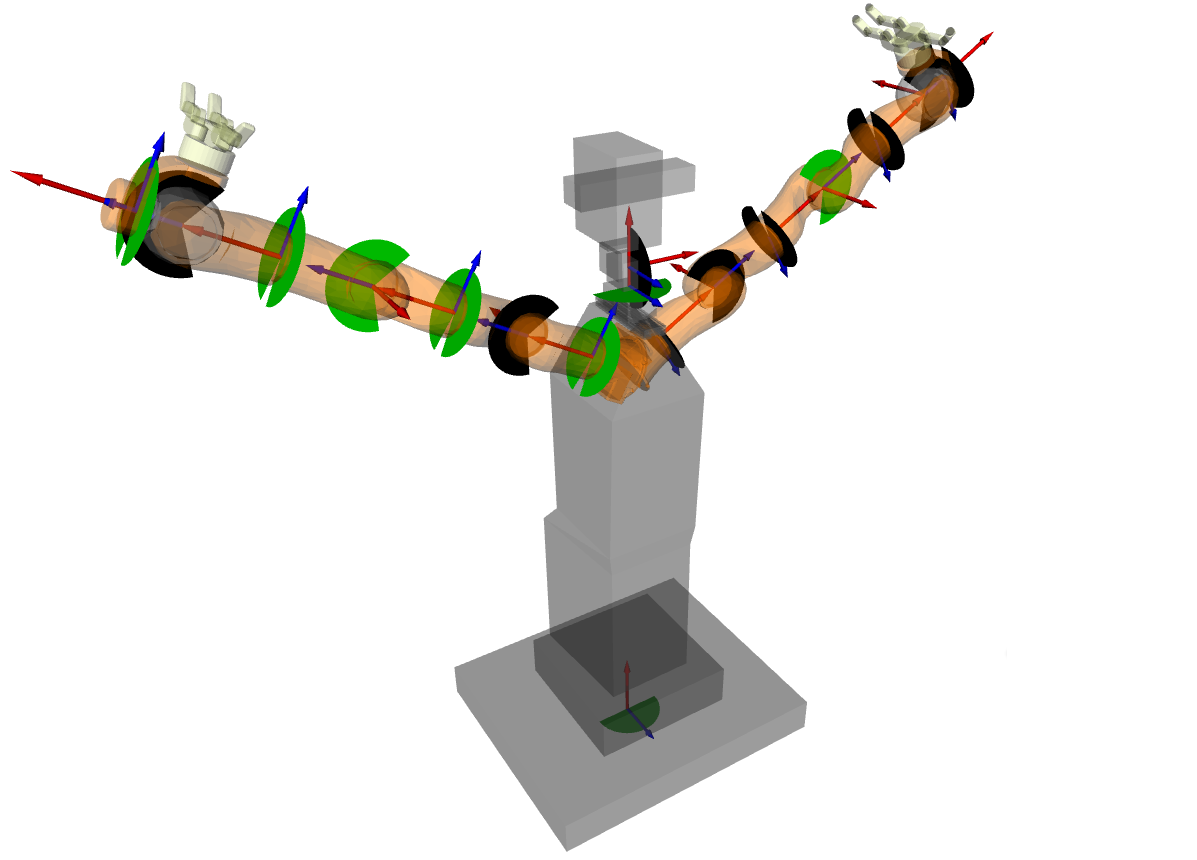
\includegraphics[scale=0.22]{./images/velma_joints.png}
\caption{Wizualizacja robota Velma z zaznaczonymi stopniami swobody \cite{docsVelma}}
\end{figure}
\end{frame}

%------------------------------------------------

\begin{frame}
\frametitle{Robot Velma}
Robot Velma składa się z \cite{docsVelma}:  
\begin{itemize}
	\item obrotowego korpusu
	\item dwóch manipulatorów KUKA LWR
	\item dwóch chwytaków BarrettHand
	\item szyi o dwóch stopniach swobody
\end{itemize}
\end{frame}

%------------------------------------------------

\begin{frame}
\frametitle{Sterowanie pozycyjne}
\begin{block}{}
Chwytaki oraz szyja robota sterowane są w sposób pozycyjny \cite{docsVelma}.
\end{block}

\begin{block}{}
Regulatory osi sterowanej kształtują prądy na podstawie różnicy pomiędzy położeniem aktualnym a zadanym.
Położenie zadane osi jest określane na podstawie wcześniej obliczonego odwrotnego zagadnienia kinematyki \cite{sterowanie}.
\end{block}

\end{frame}

%------------------------------------------------


%------------------------------------------------

\begin{frame}
\frametitle{Sterowanie pozycyjne - problem}

\begin{block}{Kontakt z otoczeniem}
W sytuacji gdy na drodze manipulatora znajdzie się przeszkoda, dążenie do zredukowania uchybu może powodować wzrost prądu
w silniku.
\end{block}

\end{frame}

%------------------------------------------------

\begin{frame}
\frametitle{Sterowanie impedancyjne}
\begin{block}{Definicja (ogólna)}
Sterowanie impedancyjne to kontrolowanie przekazywania energii do odbiornika przez zmiany nie tylko poziomu źródła ale również jego impedancji (lub admitancji). \cite{pl}.
\end{block}

\begin{block}{Definicja (robotyka, uproszczona)}
Sterowanie impedancyjne to sterownie ze zmienną sztywnością końcówki manpiulatora. 
\end{block}
\end{frame}

%------------------------------------------------

\begin{frame}
\frametitle{Sterowanie impedancyjne - robot Velma}
\begin{block}{}
Korpus oraz ramiona robota sterowane są w sposób impedancyjny (siłowy) \cite{docsVelma}.
\end{block}

\begin{block}{}
Wprowadzenie w stawach sterowania impedancyjnego zapobiega kolizji (również samokolizji) ale zmniejsza 
prawdopodobieństwo dokładnego osiągnięcia zadanej pozycji \cite{borkowska}.
\end{block}

\end{frame}

%------------------------------------------------


\subsection{Robotyka mobilna}



%------------------------------------------------
